\subsection{U-Net}\label{s:unet}
\chapterauthor{Woon Jun Wei (2200624)}

The U-Net architecture, introduced by Ronneberger et al. in 2015, is a pioneering model for biomedical image segmentation, widely adopted for various image segmentation tasks \cite{ronneberger_u-net_2015}. U-Net features a symmetric architecture with a contracting path to capture context and an expansive path for precise localization. The architecture includes skip connections that concatenate feature maps from the contracting path to the expanding path, enhancing the segmentation performance (see Figure \ref{fig:traditional_unet}).

\begin{figure}[H]
  \centering
  \begin{subfigure}[b]{0.45\textwidth}
    \centering
		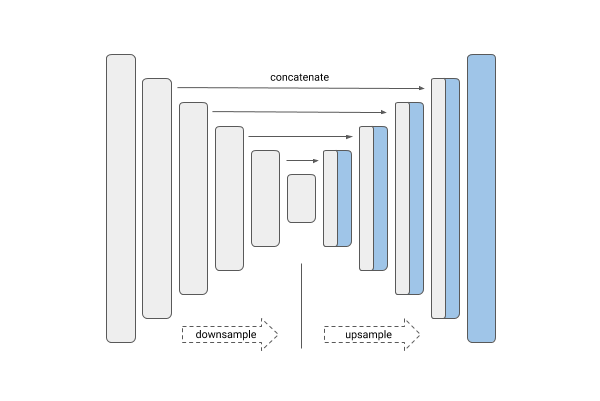
\includegraphics[width=\textwidth]{unet/unet.png}
    \caption{Traditional U-Net architecture \cite{Yakubovskiy_2019}}
    \label{fig:traditional_unet}
  \end{subfigure}
  \hfill
  \begin{subfigure}[b]{0.45\textwidth}
    \centering
		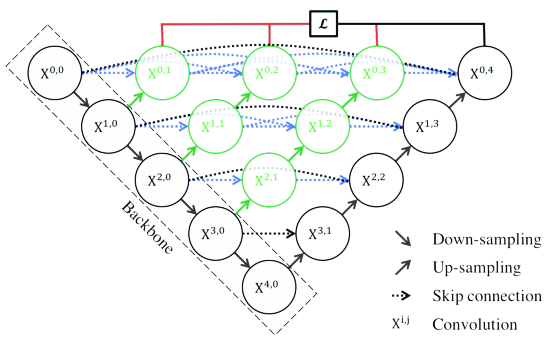
\includegraphics[width=\textwidth]{unet/unetpp.png}
    \caption{U-Net++ architecture \cite{zhou_unet_2018}}
    \label{fig:unetpp_architecture}
  \end{subfigure}
  
  \caption{U-Net and U-Net++ Architectures}\label{f:unet_vs_unetpp}
\end{figure}

Essentially, U-Net is a convolutional neural network (CNN) designed to perform image segmentation tasks by extracting features from an input image and then reconstructing the image using these extracted features. This architecture is particularly advantageous for medical image segmentation tasks, including brain tumor segmentation, where precise localization and accurate delineation of structures are critical for diagnosis and treatment planning. U-Net's unique design, with its contracting and expansive paths, allows it to capture both context and fine details, making it an ideal choice for accurately segmenting complex medical images.


\subsubsection{Implementation}

U-Net++, an extension introduced by Zhou et al. in 2018, improves the original architecture by incorporating dense skip connections (See Figure \ref{fig:unetpp_architecture}). These connections concatenate feature maps from all previous layers in the contracting path to the expanding path, enhancing feature reuse and segmentation accuracy \cite{zhou_unet_2018, zhou2019unetplusplus, zhou2018unetplusplus, zhou2021towards} (See Figure \ref{f:unet_vs_unetpp}). The U-Net++ architecture offers improved performance and efficiency compared to the original U-Net model, making it well-suited for medical image segmentation tasks.

Due to the complexity and time constraints associated with training, evaluation, and tuning, a traditional U-Net model was attempted to be architected from scratch, but was found to be infeasible within the scope of this project. Instead, this study employed the U-Net++ architecture using the \texttt{segmentation\_models} library \cite{Yakubovskiy_2019}. This library offers implementations of various deep learning models for image segmentation, supporting pre-trained models such as VGG, ResNet, and EfficientNet as down-sampling backbones.

\begin{figure}[H]
  \begin{center}
    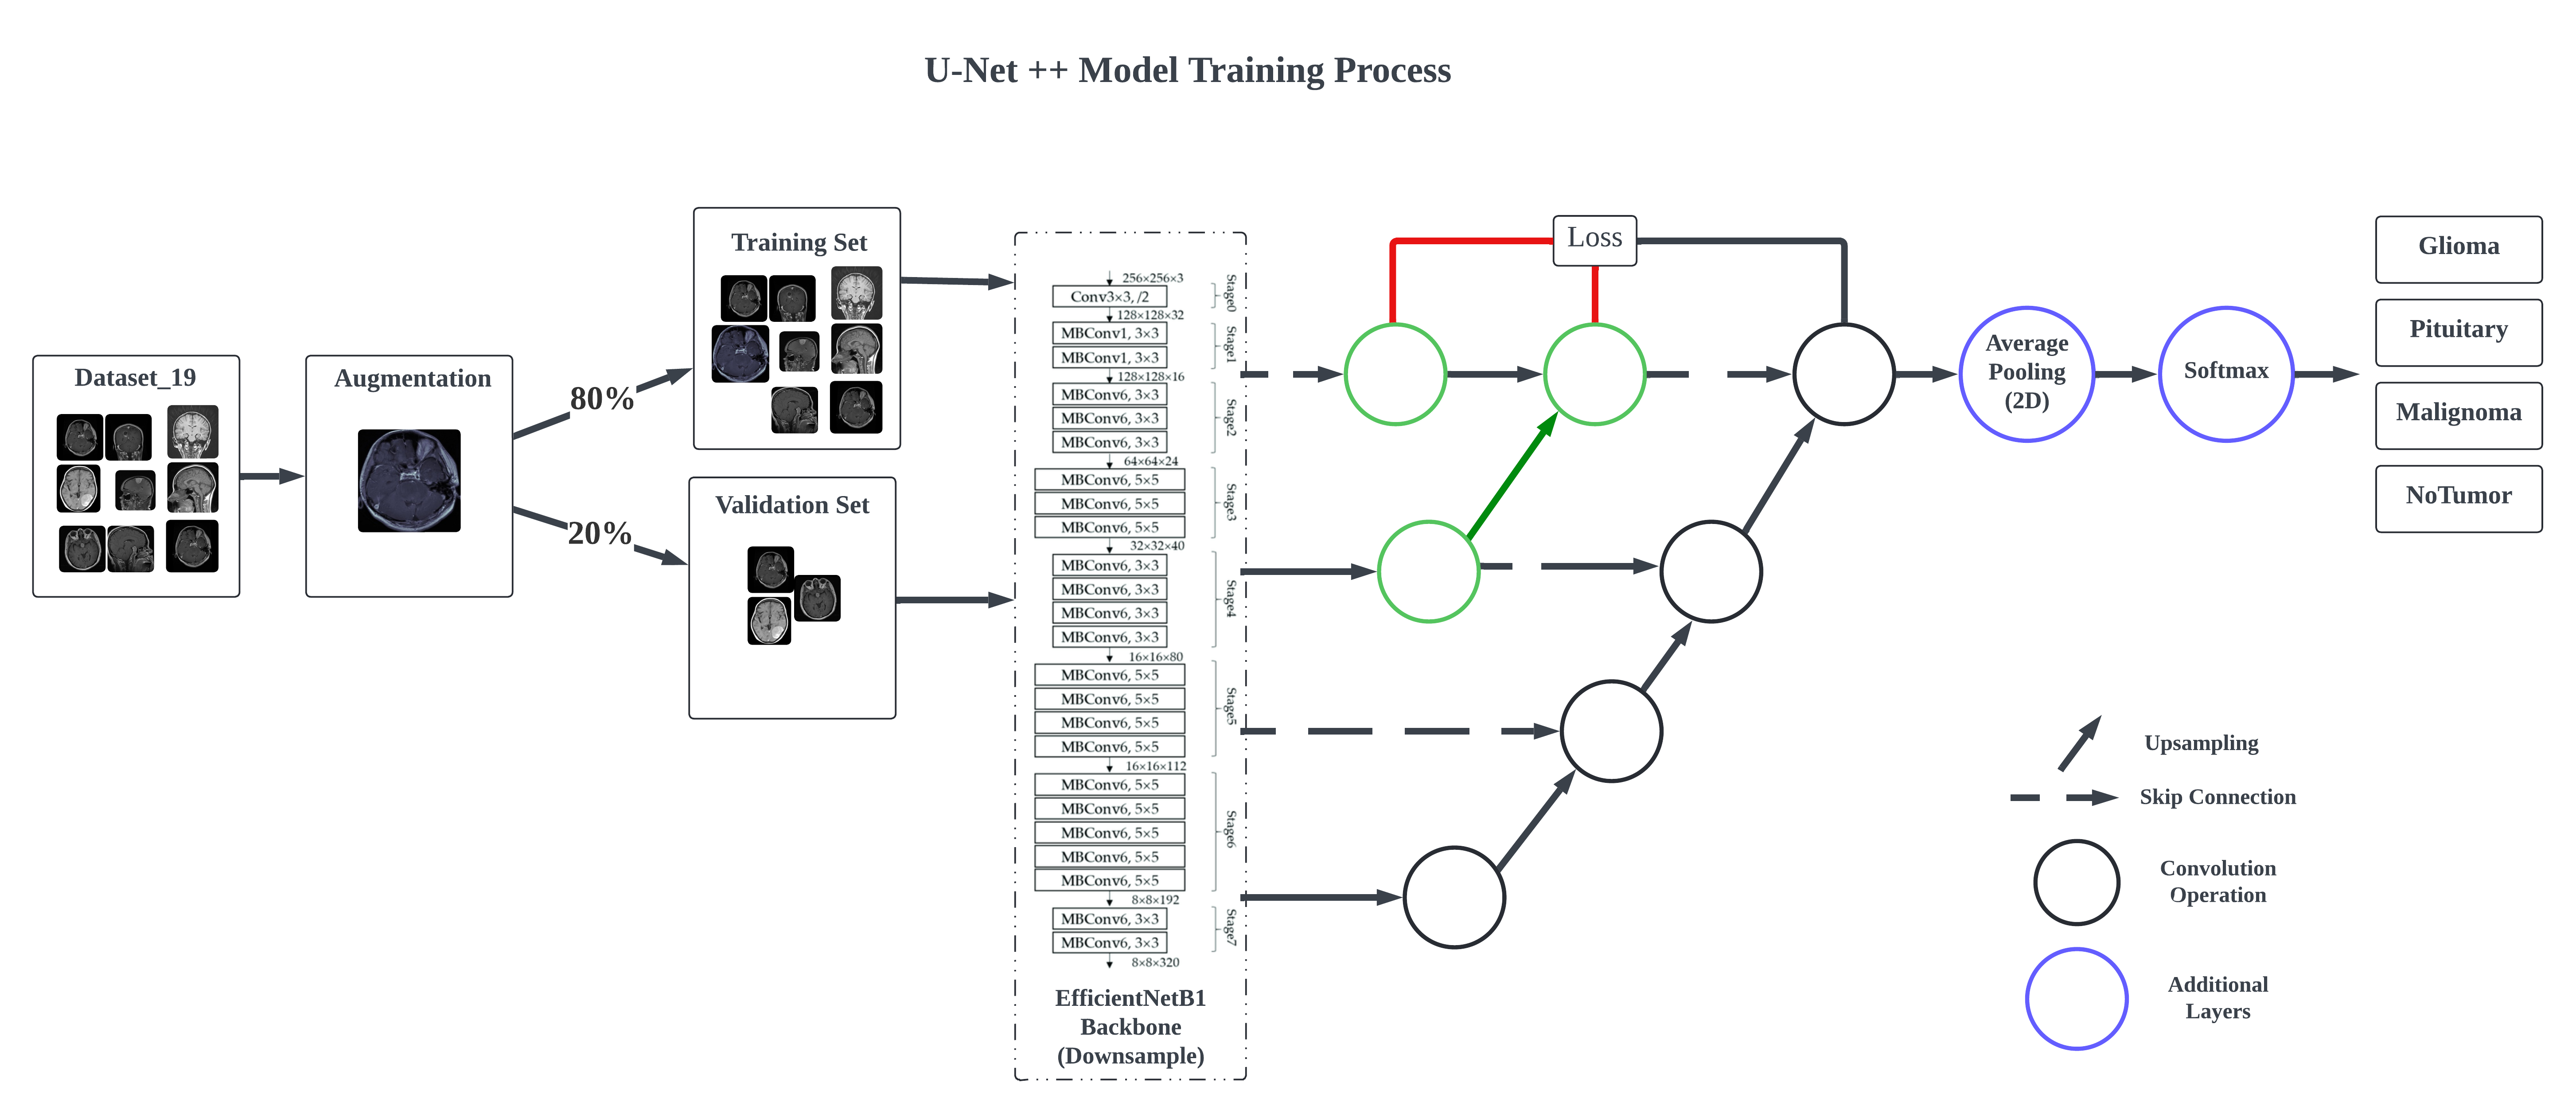
\includegraphics[width=\textwidth]{unet/unet_training.png}
  \end{center}
  \caption{U-Net++ Training Process}\label{f:unet_training}
\end{figure}

Input images were preprocessed by cropping, enhancing, and resizing to $224 \times 224 \times 3$, as detailed in Section \ref{image_cropping_enhancement}. Further preprocessing included normalization, horizontal flipping, and random rotation by 20 degrees, managed by the \texttt{ImageDataGenerator} class, which also handled the 80:20 training-validation split.

The implemented model architecture was U-Net++ with an EfficientNetB1 backbone, initialized with ImageNet weights. To obtain classification results for the full image instead of pixel-wise classification, a Global Average Pooling layer followed by a Dense layer with four units and a softmax activation function was added. The model was compiled using the categorical cross-entropy loss function and accuracy metric.

EfficientNetB1 was chosen as the backbone due to its balance between model size and performance, offering a good trade-off for the brain tumor segmentation task. EfficientNet models are known for their efficiency in terms of accuracy and computational resources, making them suitable for medical image segmentation tasks \cite{hastomo_classification_2024}. The EfficientNetB1 backbone provides a strong feature extractor while maintaining a relatively compact size, enabling efficient training and inference. Further research revealed that this approach was termed as "Eff-U-Net" in \cite{baheti_eff-unet_2020}, highlighting the effectiveness of combining EfficientNet backbones with U-Net architectures for image segmentation tasks.

The U-Net++ Model's training process is illustrated in Figure \ref{f:unet_training}, the U-Net++ Model is referenced from \cite{zhou_unet_2018}.

Training was conducted using the Adam optimizer with a learning rate of 0.0001 and a batch size of 10 for 100 epochs. The best model was saved based on validation loss, incorporating Checkpointing, Early Stopping, and Reduce Learning Rate on Plateau. Training halted at 41 epochs due to early stopping, achieving a validation loss of 0.2498 and a validation accuracy of 0.9444.

\subsubsection{Fine-Tuning}

To further optimize the performance of the U-Net++ model for brain tumor segmentation, fine-tuning was conducted using Optuna, a hyperparameter optimization framework. This process involved testing various backbone architectures to identify the most effective model configuration. The backbones evaluated included VGG16, MobileNetV2 and DenseNet121. 

The primary objective of this fine-tuning effort was to minimize the validation loss, thus enhancing the model's accuracy and generalizability. The model configuration for each trial consisted of the U-Net++ architecture with a specified backbone, followed by a Global Average Pooling layer to reduce the spatial dimensions and a Dense layer with a softmax activation function for the final classification into four classes. The models were compiled using the Adam optimizer with an initial learning rate of $1 \times 10^{-4}$, employing categorical cross-entropy as the loss function and accuracy as the performance metric.

Table \ref{tab:finetuning_results} summarizes the results of the fine-tuning trials, listing the validation loss for each tested backbone.

\begin{longtable}{|c|c|}
\caption{Fine-Tuning Results for Different Backbones}\label{tab:finetuning_results} \\
\hline
\textbf{Backbone} & \textbf{Validation Loss} \\
\hline
\endfirsthead

\multicolumn{2}{c}{{\bfseries \tablename\ \thetable{} -- continued from previous page}} \\
\hline
\textbf{Backbone} & \textbf{Validation Loss} \\
\hline
\endhead

\hline \multicolumn{2}{|r|}{{Continued on next page}} \\ \hline
\endfoot

\hline
\endlastfoot

MobileNetV2 (Trial 1) & 0.4158 \\
\hline
DenseNet121 (Trial 2) & 0.3684 \\
\hline
MobileNetV2 (Trial 3) & 0.7039 \\
\hline
VGG16 (Trial 4) & 0.7004 \\
\end{longtable}


The Optuna optimization process involved creating a model with a backbone suggested by Optuna for each trial. Each model was then trained for 35 epochs using the Adam optimizer, with callbacks for learning rate reduction, early stopping, and model checkpointing based on validation loss. The best validation loss achieved during training was recorded as the objective metric for each trial.

While DenseNet121 achieved the lowest validation loss of 0.3684 during the fine-tuning trials, it was observed that the EfficientNetB1 backbone, used during the initial training phase, demonstrated superior performance with a lower validation loss and higher accuracy. Specifically, the EfficientNetB1 model achieved a validation loss of 0.2498 and a validation accuracy of 0.9444, outperforming the DenseNet121 in terms of both loss and accuracy metrics. Consequently, despite the promising results from DenseNet121, EfficientNetB1 was retained as the preferred backbone for the final U-Net++ model due to its demonstrated efficacy and robust performance during the training phase.

The fine-tuning process underscored the significance of backbone selection in enhancing the model's performance. Although DenseNet121 showed potential with the lowest validation loss among the tested backbones, EfficientNetB1 was ultimately chosen for its superior overall performance, contributing to the model's effectiveness in accurately segmenting brain tumors. The results are summarized in Table \ref{tab:finetuning_results}.

\subsubsection{Results and Evaluation}

\begin{figure}[H]
  \centering
  \begin{subfigure}[b]{0.2\textwidth}
    \centering
    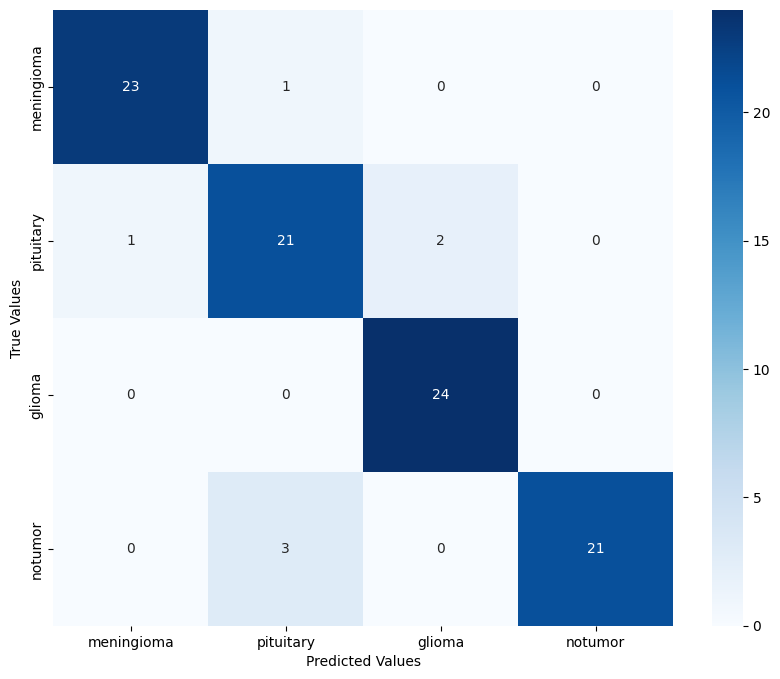
\includegraphics[width=\textwidth]{unet/evaluation/cm1.png}
    \caption{Confusion Matrix}
    \label{fig:unet_cm1}
  \end{subfigure}
  \hfill
  \begin{subfigure}[b]{0.2\textwidth}
    \centering
    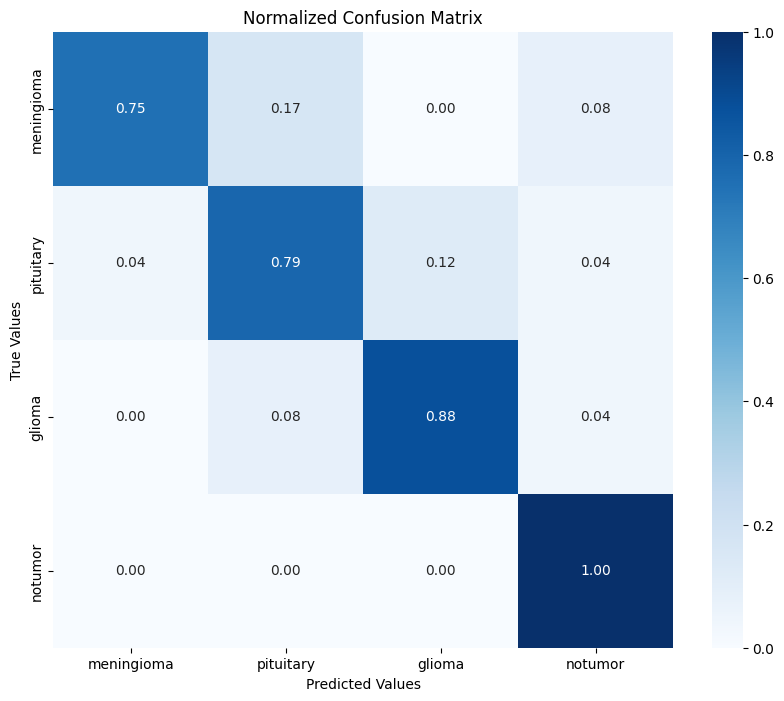
\includegraphics[width=\textwidth]{unet/evaluation/cm2.png}
    \caption{Normalized Confusion Matrix}
    \label{fig:unet_cm2}
  \end{subfigure}
  \hfill
  \begin{subfigure}[b]{0.25\textwidth}
    \centering
    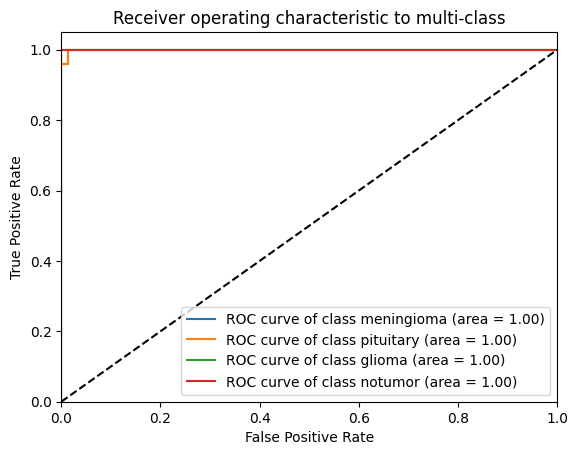
\includegraphics[width=\textwidth]{unet/evaluation/ROC.png}
    \caption{ROC Curve}
    \label{fig:unet_roc}
  \end{subfigure}
  \hfill
  \begin{subfigure}[b]{0.25\textwidth}
    \centering
    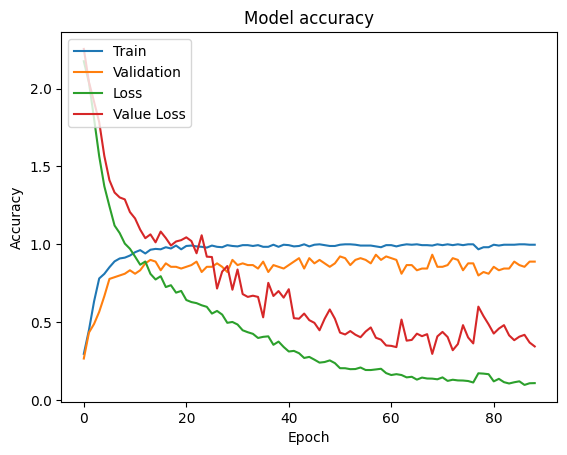
\includegraphics[width=\textwidth]{unet/evaluation/learning_curve.png}
    \caption{Learning Curve}
    \label{fig:unet_learning_curve}
  \end{subfigure}
  \caption{Confusion Matrix, Normalized Confusion Matrix, ROC Curve, and Learning Curve for Brain Tumor Segmentation}
  \label{fig:unet_evaluation}
\end{figure}

\begin{table}[ht]
\centering
\begin{tabular}{cc}
    \begin{minipage}{.6\linewidth}
        \centering
        \begin{subtable}[t]{\linewidth}
            \centering
            \begin{tabular}{|l|c|c|c|c|}
                \hline 
                \textbf{Class} & \textbf{Precision} & \textbf{Recall} & \textbf{F1-Score} & \textbf{Support} \\ 
                \hline 
                meningioma & 0.95 & 0.88 & 0.91 & 24 \\ 
                \hline
                pituitary  & 0.88 & 0.92 & 0.90 & 24 \\ 
                \hline
                glioma     & 0.96 & 1.00 & 0.98 & 24 \\ 
                \hline
                notumor    & 0.96 & 0.96 & 0.96 & 24 \\ 
                \hline
                micro avg  & 0.94 & 0.94 & 0.94 & 96 \\ 
                \hline
                macro avg  & 0.94 & 0.94 & 0.94 & 96 \\ 
                \hline
                weighted avg & 0.94 & 0.94 & 0.94 & 96 \\ 
                \hline
                samples avg & 0.94 & 0.94 & 0.94 & 96 \\ 
                \hline
            \end{tabular}
            \caption{Classification Report for Brain Tumor Segmentation} 
            \label{tab:unet_classification_report}
        \end{subtable}
    \end{minipage} &
    \begin{minipage}{.35\linewidth}
        \centering
        \begin{subtable}[t]{\linewidth}
            \centering
            \begin{tabular}{|c|c|}
                \hline 
                \textbf{Metric} & \textbf{Value} \\ 
                \hline
                DSC & 0.9372 \\ 
                \hline
                Sensitivity & 0.9375 \\ 
                \hline
                Specificity & 0.9792 \\ 
                \hline
                Accuracy & 0.9375 \\ 
                \hline
            \end{tabular}
            \caption{Additional Metrics for Brain Tumor Segmentation} 
            \label{tab:unet_additional_metrics}
        \end{subtable}
    \end{minipage}
\end{tabular}
\caption{Classification Report and Additional Metrics for Brain Tumor Segmentation}
\label{tab:combined_metrics}
\end{table}


The performance metrics presented in Tables \ref{tab:unet_classification_report} and \ref{tab:unet_additional_metrics} demonstrate the robust capability of the U-Net model in brain tumor segmentation. The classification report (Table \ref{tab:unet_classification_report}) highlights the model's high precision, recall, and F1-scores across all classes, with an overall accuracy of 0.94. Specifically, the model achieved precision scores of 0.96, 0.91, 0.92, and 0.96 for the meningioma, pituitary, glioma, and notumor classes, respectively. Corresponding recall values were 0.92, 0.88, 1.00, and 0.96, indicating the model's effectiveness in identifying true positives for each class.

The confusion matrix in Figure \ref{fig:unet_cm1} provides a visual representation of the model's classification accuracy, revealing a minimal number of misclassifications. The ROC Curve in Figure \ref{fig:unet_roc} further substantiates the model's excellent performance, demonstrating a strong ability to distinguish between different classes. 

Additional evaluation metrics in Table \ref{tab:unet_additional_metrics} confirm the model's robustness. The Dice Similarity Coefficient (DSC) of 0.9370 indicates a high overlap between the predicted and actual tumor regions, underscoring the model's precise segmentation capabilities. Sensitivity and specificity values of 0.9375 and 0.9792, respectively, further highlight the model's accuracy in detecting tumor presence while minimizing false positives.

Mentioned in \cite{abd-ellah_automatic_2024}, the varying nature and size of glioma tumors pose significant challenges for accurate segmentation. Despite these challenges, the U-Net model achieved an impressive F1-score of 0.96 for glioma, indicating a low incidence of false positives and false negatives. This performance suggests that the model is highly effective in segmenting glioma tumors, although there remains potential for further improvement. Fine-tuning the model or employing additional data augmentation techniques could enhance the segmentation accuracy for glioma tumors, thereby improving overall model performance.

\subsubsection{K-Folds Cross-Validation}

\begin{figure}[H]
  \begin{center}
    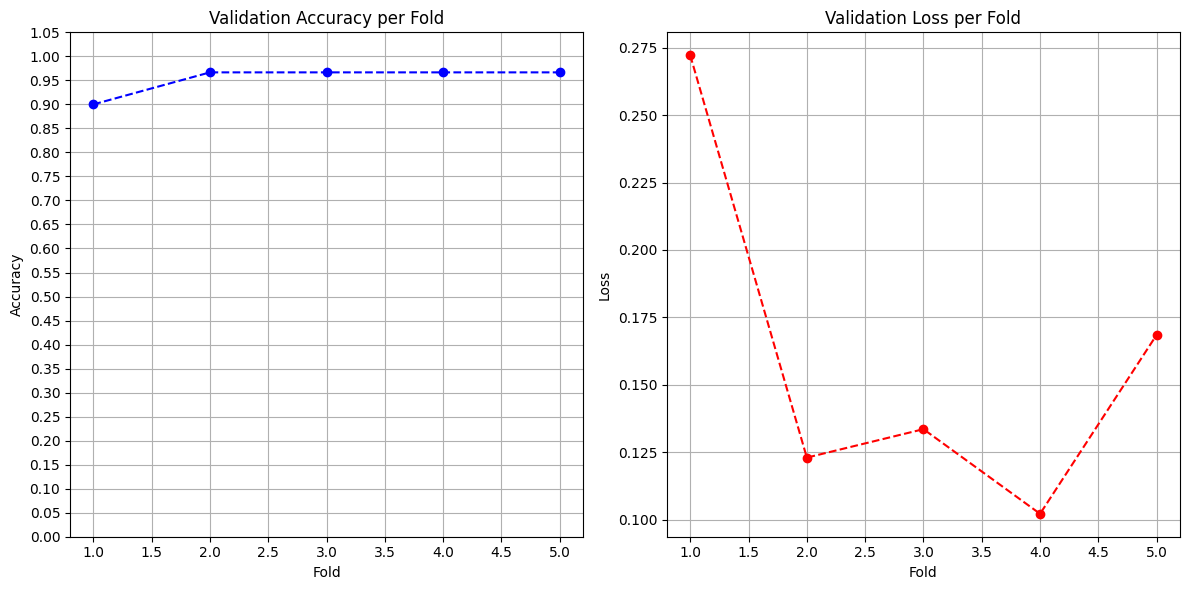
\includegraphics[width=0.5\textwidth]{unet/evaluation/kfolds.png}
  \end{center}
  \caption{K-Folds Cross-Validation for Brain Tumor Segmentation}\label{f:unet_kfolds}
\end{figure}

K-Folds cross-validation was conducted to rigorously assess the model's generalization performance on the brain tumor segmentation task. The dataset was partitioned into five folds, ensuring each fold served as the validation set exactly once while the remaining four folds were utilized for training. This procedure was repeated five times, allowing each fold to be used for validation, thus providing a robust estimate of the model's performance. The model was trained for 35 epochs for each fold, with the initial training stopping at 33 epochs due to early stopping. Model checkpoints were removed for efficiency during this process.

The left plot in Figure \ref{f:unet_kfolds} illustrates the validation accuracy for each fold. The accuracy values per fold indicate high performance across all splits, with a slight variation. Specifically, the accuracy ranged from approximately 0.90 to 1.00, demonstrating the model's strong capability in accurately segmenting brain tumors. This high level of accuracy across different folds suggests that the model generalizes well to unseen data, maintaining its performance across various subsets of the dataset.

The right plot in Figure \ref{f:unet_kfolds} presents the validation loss for each fold. The loss values show greater variability compared to the accuracy, with the highest loss observed in fold 1 and the lowest in fold 4. The variability in the loss values suggests that while the model generally performs well, there are certain instances where the model's performance can be further optimized. This indicates potential areas for improvement, particularly in achieving more consistent performance across different validation sets.

It is noteworthy that during the K-Folds validation, there were instances where the validation loss was smaller than the training's validation loss, and the accuracy during K-Folds was also higher. This phenomenon underscores the model's robustness, indicating that it is capable of performing well on unseen data. However, this occurrence may also be attributed to the differences in data distribution between the training and validation sets in each fold. This disparity can sometimes lead to lower validation loss and higher accuracy, suggesting that while the model is strong, the evaluation metrics might slightly overestimate the model's performance. Therefore, it is important to consider these factors when interpreting the results.

Overall, the K-Folds cross-validation results indicate that the model achieves a high average accuracy of 0.9533 with a standard deviation of 0.0267, reflecting robust performance with minimal variability. The average validation loss was 0.1599 with a standard deviation of 0.0601, suggesting that while the model's predictions are generally reliable, there is room for enhancement in terms of reducing the prediction error. These metrics collectively demonstrate that the model possesses strong generalization capabilities, although further refinement could help in achieving even greater consistency and reliability in its performance. The metrics and conditions for K-Folds cross-validation are summarized in Table \ref{tab:unet_kfolds_combined}.

\begin{table}[H]
\centering
\begin{tabular}{cc}
    \begin{minipage}{.45\linewidth}
        \centering
        \begin{subtable}[t]{\linewidth}
            \centering
            \begin{tabular}{|l|c|}
                \hline
                \textbf{Metric} & \textbf{Value} \\
                \hline
                Average Validation Accuracy & 0.9533 \\
                \hline
                Accuracy Std. Dev. & 0.0267 \\
                \hline
                Average Validation Loss & 0.1599 \\
                \hline
                Loss Std. Dev. & 0.0601 \\
                \hline
            \end{tabular}
            \caption{Evaluation Metrics}
        \end{subtable}
    \end{minipage} &
    \begin{minipage}{.45\linewidth}
        \centering
        \begin{subtable}[t]{\linewidth}
            \centering
            \begin{tabular}{|l|c|}
                \hline
                \textbf{Parameter} & \textbf{Value} \\
                \hline
                Number of Folds & 5 \\
                \hline
                Epochs per Fold & 35 \\
                \hline
                Batch Size & 10 \\
                \hline
            \end{tabular}
            \caption{Testing Conditions}
        \end{subtable}
    \end{minipage}
\end{tabular}
\caption{K-Folds Cross-Validation Metrics and Conditions for Brain Tumor Segmentation}\label{tab:unet_kfolds_combined}
\end{table}

\subsubsection{Semantic Segmentation Analysis}

The segmentation results using the U-Net model for brain tumor classification offer critical insights into the model's learning and performance. The U-Net architecture, known for its effectiveness in biomedical image segmentation, was anticipated to accurately delineate brain tumor boundaries. To assess the model's segmentation performance, we visualized its predictions by overlaying the segmentation mask on the original images. This process involved generating a binary mask from the U-Net model's predictions using a threshold value of 0.9, and then overlaying this mask on the original images to highlight the segmented regions.

It is important to note that the model was not trained with explicit tumor masks. Instead, this attempt aims to illustrate what the model identifies as "important features" for classification. This approach helps to understand the regions the model considers significant in distinguishing different classes of brain tumors, thereby providing insights into the model's decision-making process.

Given the pixel-wise prediction probabilities $\mathbf{P}_i$ (From U-Net's Final Layer) for the $i$-th image, we define $\mathbf{P}_i$ as:
\[
\mathbf{P}_i = \text{model.predict}(x_i)
\]
where $x_i$ is the input image. Here, $\mathbf{P}_i$ is a tensor of shape $(H, W, C)$, where $H$ and $W$ are the height and width of the image, and $C$ is the number of classes.

For a specific class $c$, the pixel-wise probability map $\mathbf{P}_{i,c}$ is extracted as:
\[
\mathbf{P}_{i,c} = \mathbf{P}_i[:, :, c]
\]
To create a binary mask for class $c$, we apply a threshold $\tau$ to $\mathbf{P}_{i,c}$:
\[
\text{mask}_{i,j,c} = 
\begin{cases} 
1 & \text{if } \mathbf{P}_{i,c}(j,k) > \tau \\
0 & \text{otherwise}
\end{cases}
\]
where $\mathbf{P}_{i,c}(j,k)$ is the probability of pixel $(j,k)$ belonging to class $c$.

The binary mask $\mathbf{M}_{i,c}$ for class $c$ thus becomes:
\[
\mathbf{M}_{i,c}(j,k) = \text{mask}_{i,j,c}
\]
where $\mathbf{M}_{i,c}$ is a binary matrix of shape $(H, W)$ indicating the presence of class $c$ at each pixel.

The binary mask $\mathbf{M}_{i,c}$ is overlayed onto the original image $\mathbf{I}$ to highlight regions of interest. The overlay process can be described as follows:
\[
\mathbf{I}'(j,k) = 
\begin{cases} 
(0, 255, 0) & \text{if } \mathbf{M}_{i,c}(j,k) = 1 \\
\mathbf{I}(j,k) & \text{otherwise}
\end{cases}
\]
where $\mathbf{I}'$ is the resulting image with the overlay, showing the masked areas in green (RGB value (0, 255, 0)).

By combining all the pixels that belong to class $c$, the segmentation mask effectively highlights the regions of interest corresponding to that class in the original image. The Algorithm used for image prediction and visualization with mask overlay is provided in Algorithm \ref{alg:unet_visualization} (See Appendix \ref{ss:segmentationAlgorithm}).

\begin{figure}[H]
  \centering
  \begin{subfigure}[b]{0.23\textwidth}
    \centering
    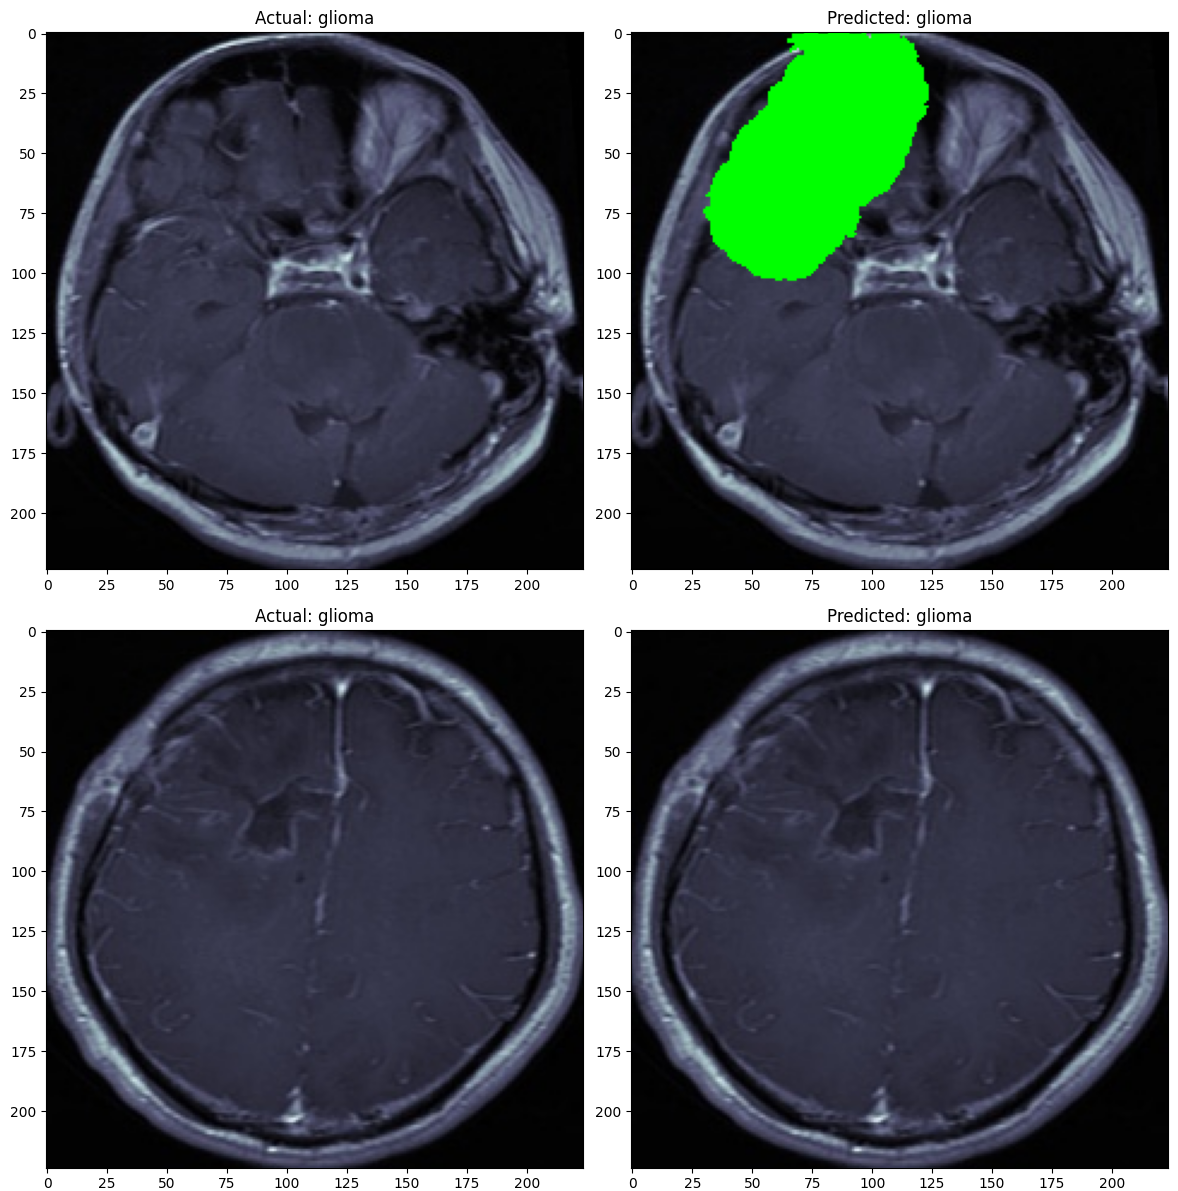
\includegraphics[width=\textwidth]{unet/evaluation/segmentation1.png}
    \caption{Glioma}
    \label{fig:glio_seg}
  \end{subfigure}
  \hfill
  \begin{subfigure}[b]{0.23\textwidth}
    \centering
    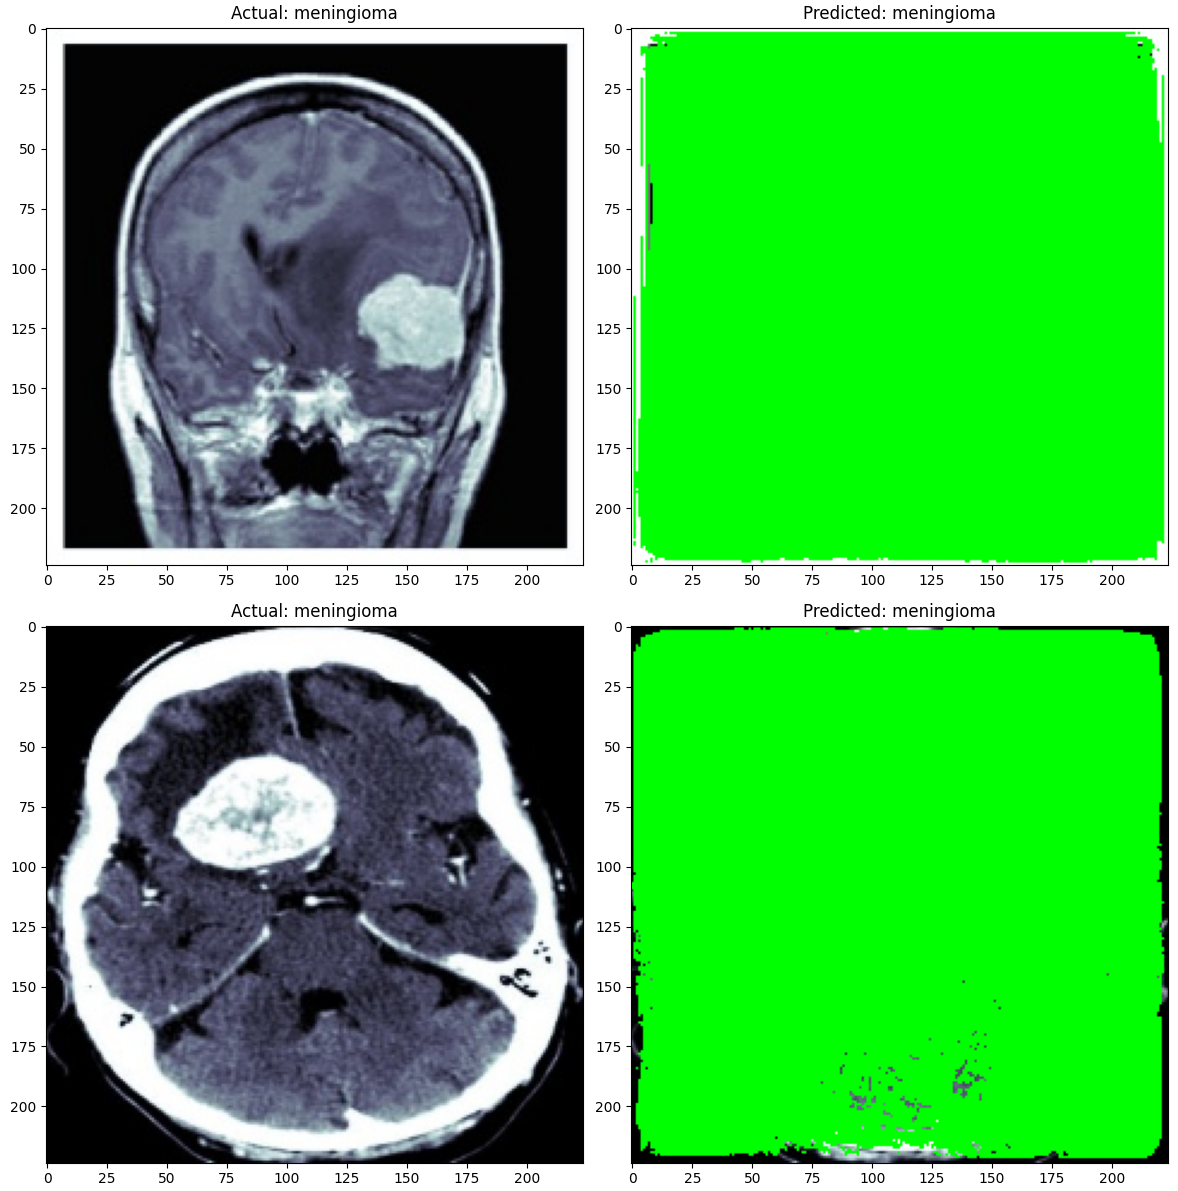
\includegraphics[width=\textwidth]{unet/evaluation/segmentation2.png}
    \caption{Menigioma}
    \label{fig:meng_seg}
  \end{subfigure}
  \hfill
  \begin{subfigure}[b]{0.23\textwidth}
    \centering
    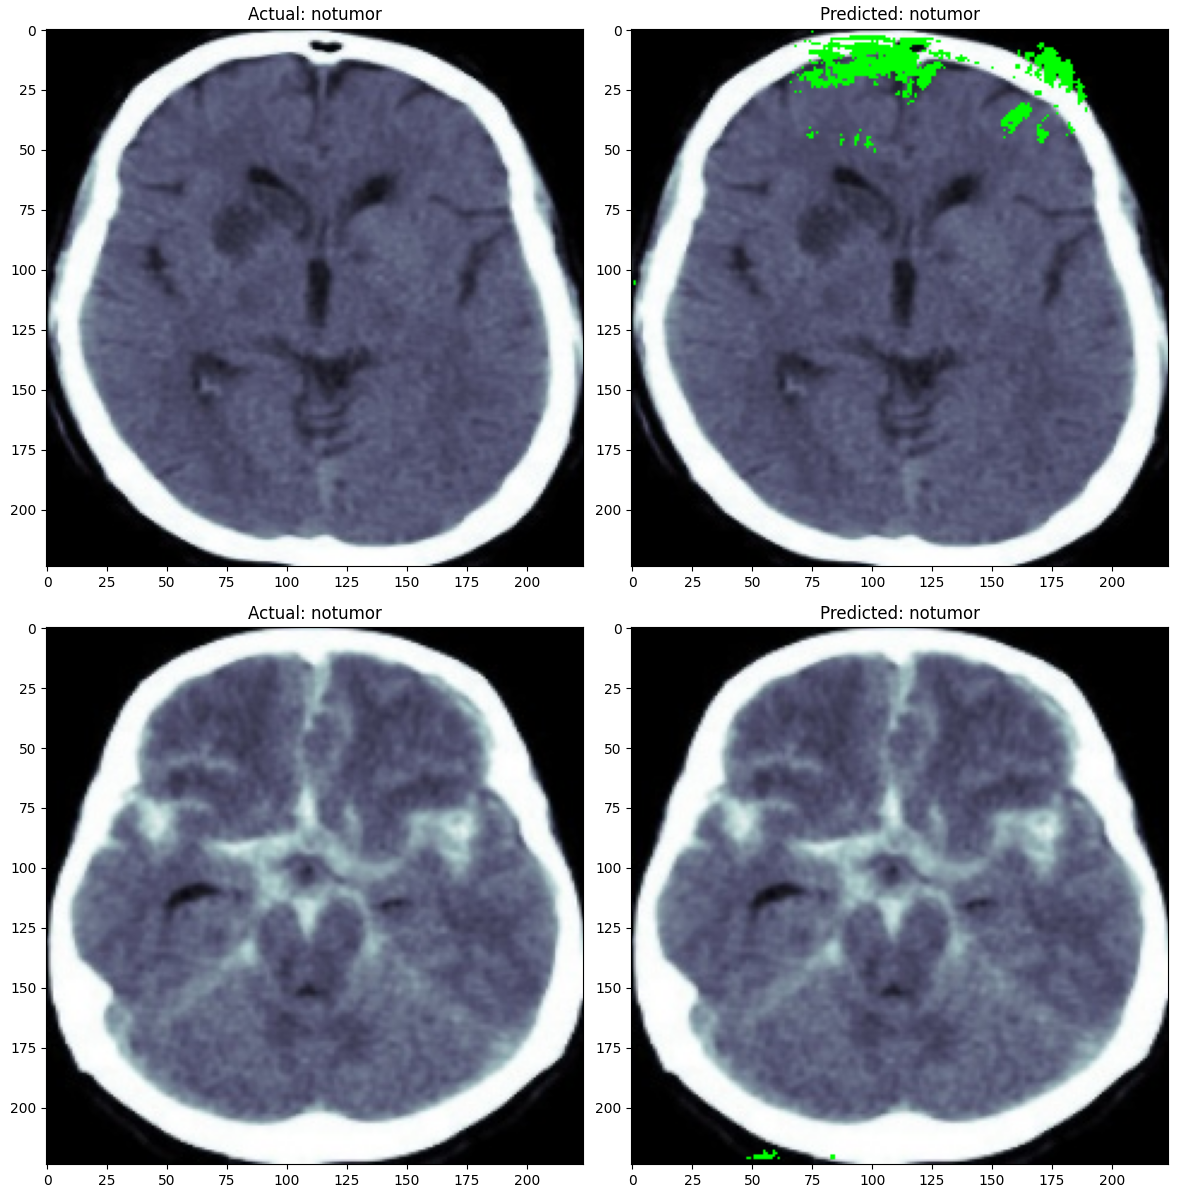
\includegraphics[width=\textwidth]{unet/evaluation/segmentation3.png}
    \caption{No Tumor}
    \label{fig:no_tumor_seg}
  \end{subfigure}
  \hfill
  \begin{subfigure}[b]{0.23\textwidth}
    \centering
    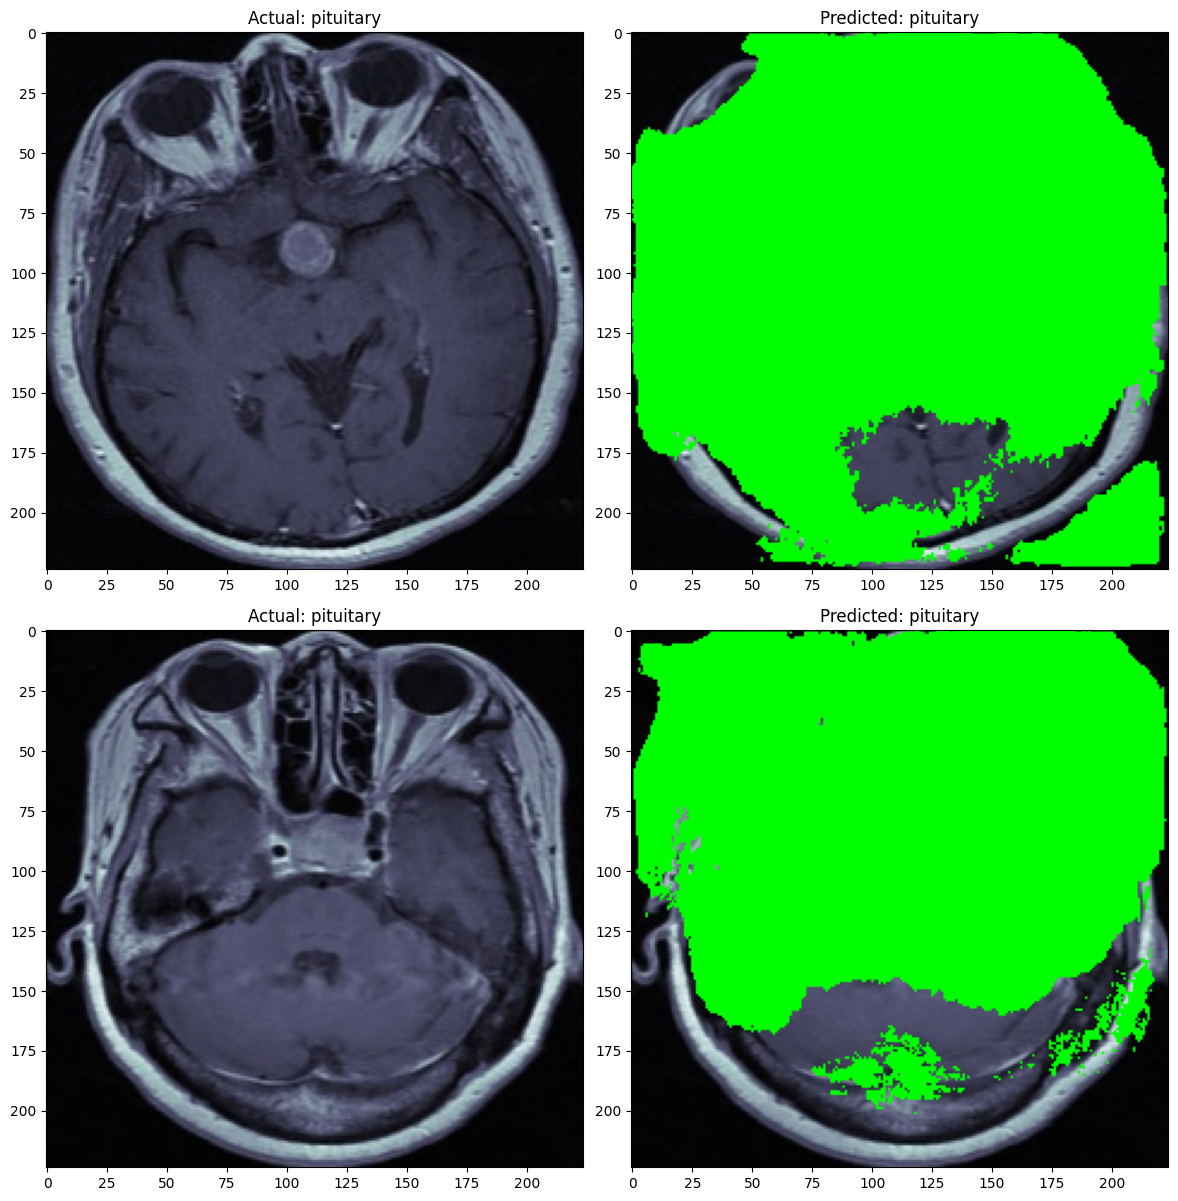
\includegraphics[width=\textwidth]{unet/evaluation/segmentation4.png}
    \caption{Pituitary}
    \label{fig:pitu_seg}
  \end{subfigure}
  \caption{Segmentation Results for Brain Tumor Classes (Original (Left) vs Masked (Right))}
  \label{fig:segmentation_results}
\end{figure}

\begin{figure}[H]
  \centering
  \begin{subfigure}[b]{0.23\textwidth}
    \centering
    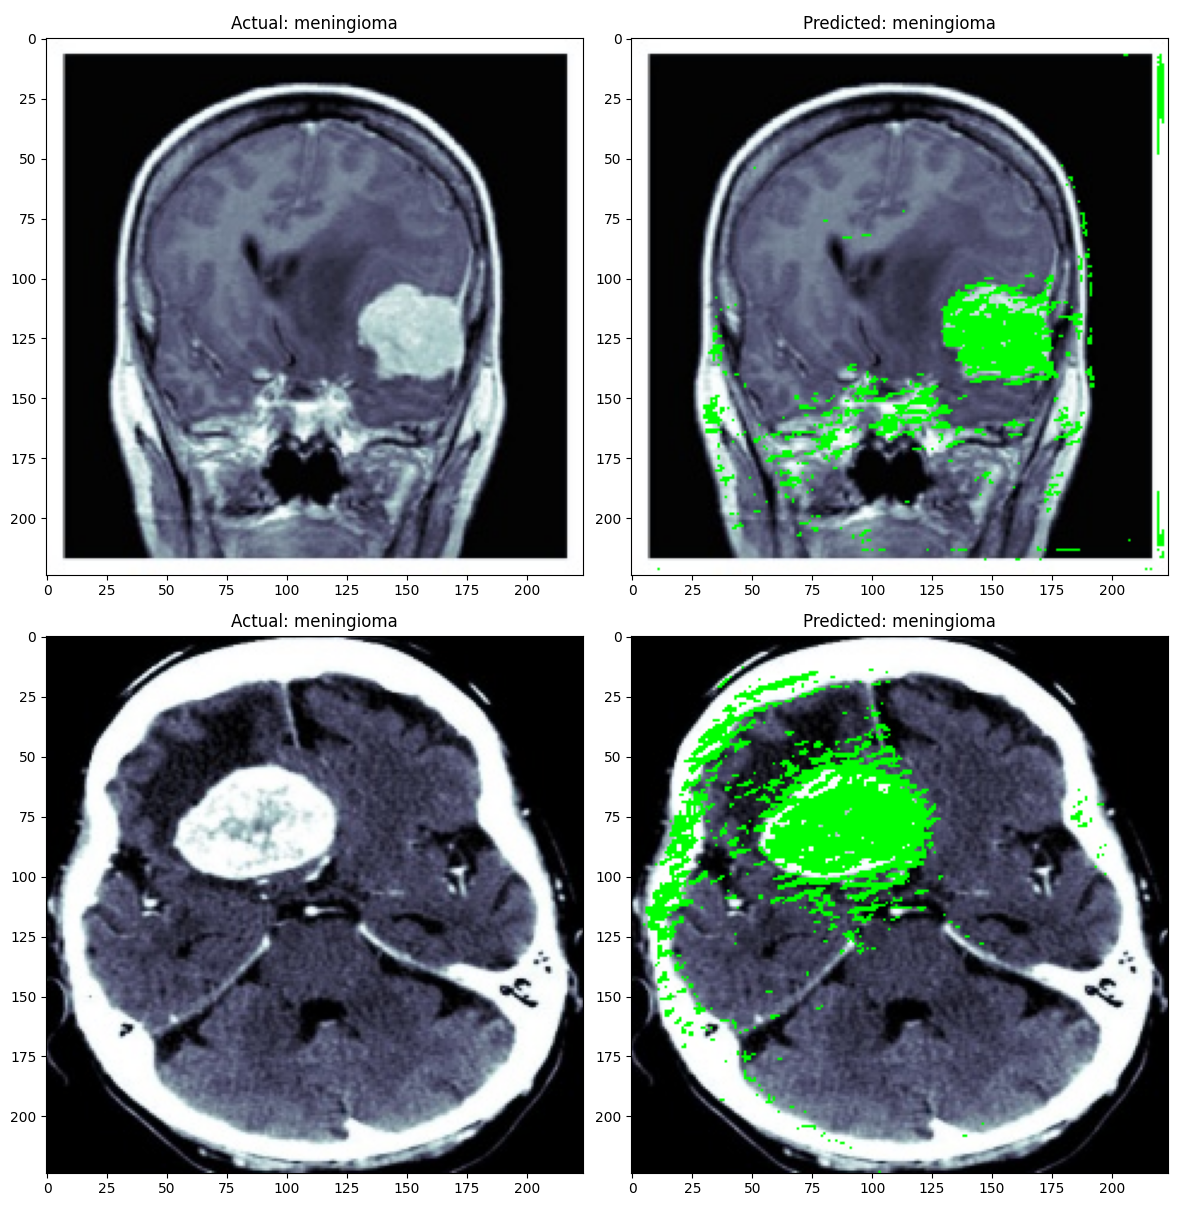
\includegraphics[width=\textwidth]{unet/evaluation/meningioma_1.png}
    \caption{Menigioma Segmentation Attempt 2}
    \label{fig:meningioma_1}
  \end{subfigure}
  \begin{subfigure}[b]{0.23\textwidth}
    \centering
    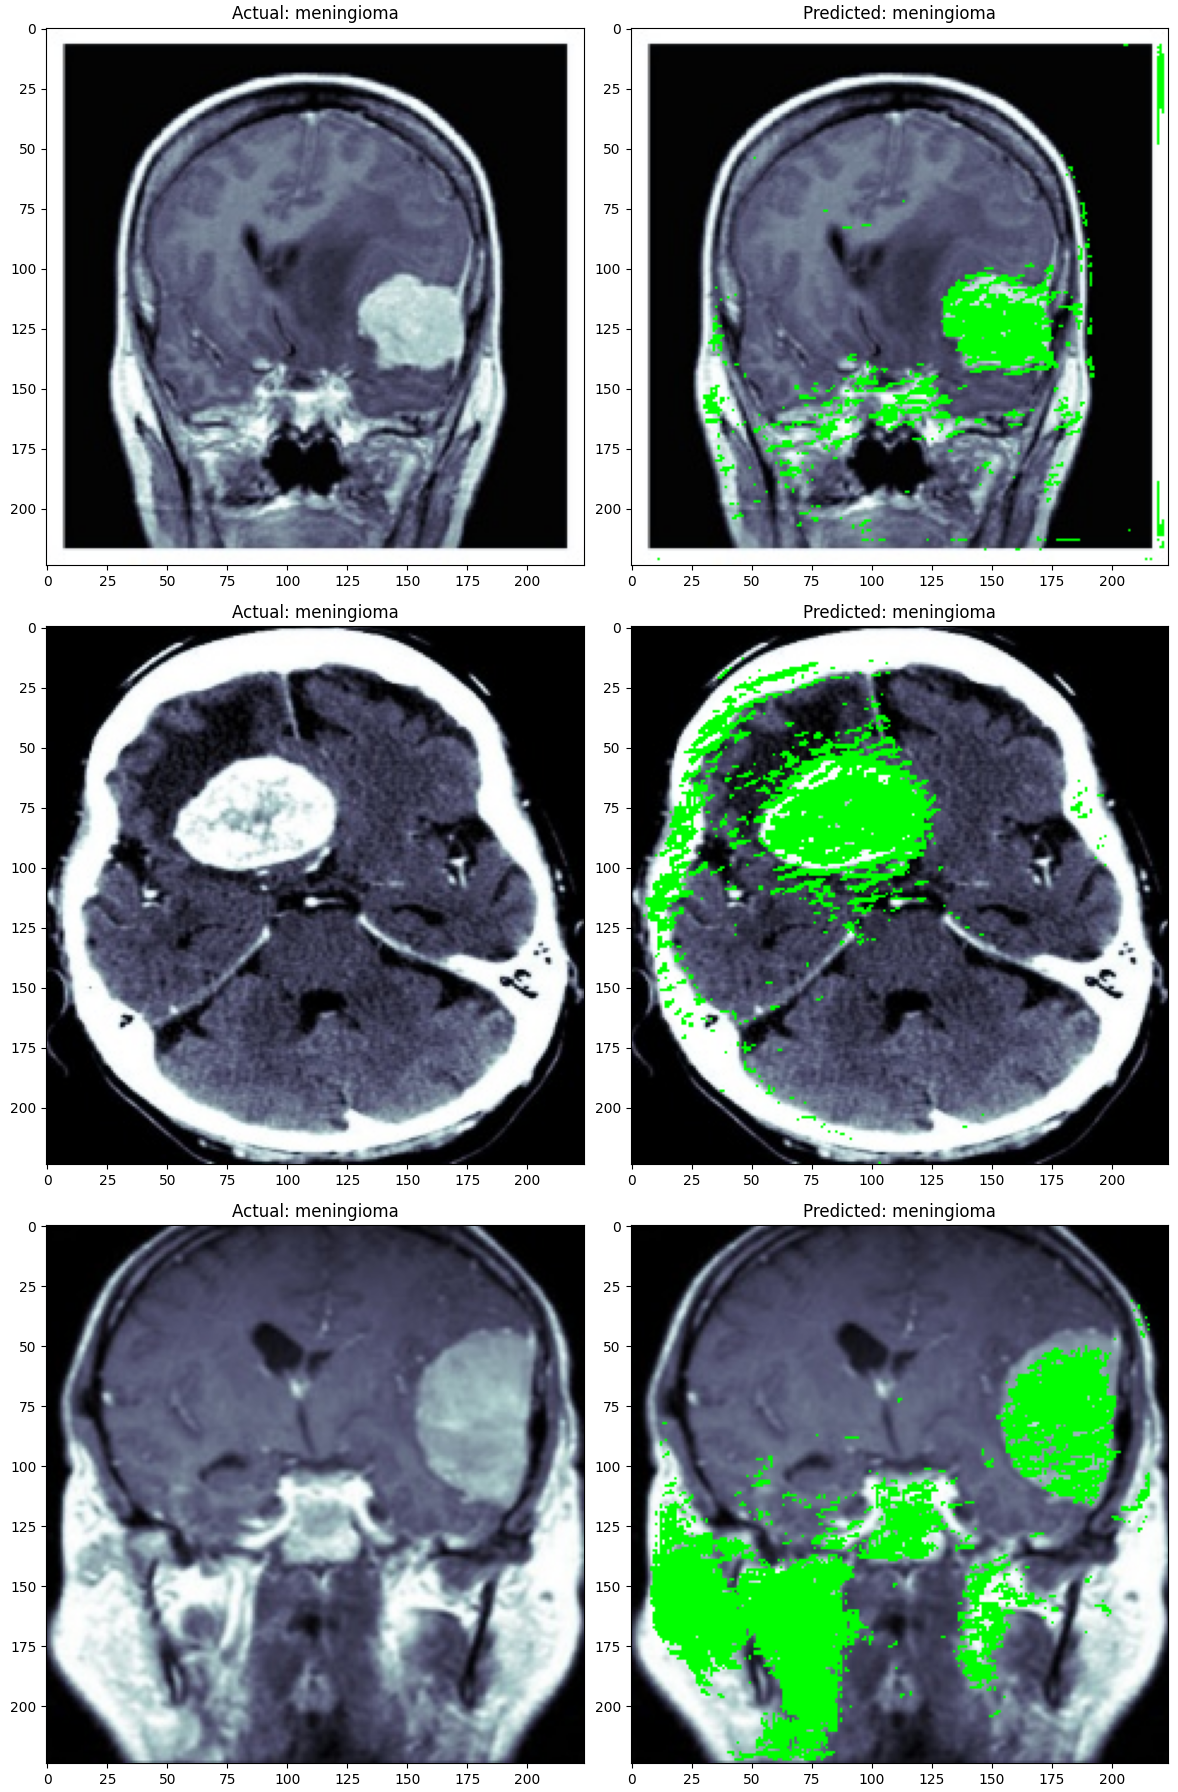
\includegraphics[width=\textwidth]{unet/evaluation/meningioma_2.png}
    \caption{Menigioma Segmentation Attempt 3}
    \label{fig:mengioma_2}
  \end{subfigure}
  \caption{Additional Segmentation Results for Menigioma (Original (Left) vs Masked (Right))}
  \label{fig:meningioma_segmentation}
\end{figure}


The segmentation results using the U-Net model for brain tumor classification provide valuable insights into the model's learning and performance. The U-Net architecture, renowned for its efficacy in biomedical image segmentation, was anticipated to accurately delineate brain tumor boundaries. However, the results obtained with a threshold of 0.9 applied to the model's output reveal several discrepancies.

As illustrated in Figure \ref{fig:segmentation_results}, the model frequently segments regions that do not correspond to actual tumor locations. For instance, in glioma cases, the model identifies brain regions that do not align with the actual tumor areas. Similarly, for images labeled as having no tumor, the model erroneously segments parts of the brain, suggesting that it has learned features unrelated to tumor presence. This observation indicates that the model has predominantly learned to segment brain regions rather than tumors themselves.

The segmentation mask for meningioma shows high confidence across the entire image (see Figure \ref{fig:meng_seg}), resulting in over-segmentation. Similarly, the pituitary tumor segmentation mask covers a large portion of the image, indicating an overestimation of the tumor area. This over-coverage arises from the model's inability to accurately differentiate between tumor and non-tumor regions when the threshold is set too high, thus compromising segmentation specificity. Additional testing revealed that the model can segment meningioma tumors with high accuracy, as shown in Figure \ref{fig:meningioma_segmentation}. The model successfully identifies the tumor regions and provides precise segmentation results, demonstrating its capability in accurately delineating meningioma tumors. Additional images are provided in Appendix \ref{s:unetAppendix}.

Several factors contribute to this misalignment. One significant factor is the inadequacy of the training dataset in terms of size and diversity, leading to poor generalization. A limited dataset restricts the model's exposure to the varied appearances and characteristics of tumors, impairing its ability to learn robust, tumor-specific features.

Conversely, for images labeled as having no tumor, the model segments only small portions of the image. While this suggests that the model can sometimes correctly identify non-tumor regions, it struggles with precise localization and segmentation, resulting in scattered and incomplete outputs.

Moreover, the absence of explicit tumor masks in the training data presents a significant challenge. Without precise annotations indicating tumor boundaries, the model struggles to differentiate between tumor and non-tumor regions effectively. This underscores the need for a more comprehensive dataset with detailed tumor masks to enhance segmentation accuracy.

While the U-Net model demonstrates some capability in learning from the given dataset, its performance in accurately segmenting brain tumors is suboptimal. The results emphasize the need for a larger and more detailed dataset, specifically annotated with tumor masks, to improve the model's ability to identify and segment tumors accurately. Future work should focus on augmenting the dataset and incorporating advanced training techniques to address these limitations and achieve more reliable segmentation outcomes.

\subsubsection{Conclusion}\label{s:conclusion}

In this study, we implemented and fine-tuned the U-Net++ model for the challenging task of brain tumor segmentation, utilizing various backbone architectures. Our comprehensive approach involved initial training with the EfficientNetB1 backbone, followed by fine-tuning with alternative backbones such as VGG16, MobileNetV2, and DenseNet121. The EfficientNetB1 backbone demonstrated superior performance, achieving a validation loss of 0.1862 and a validation accuracy of 0.9444. This backbone was retained for the final model due to its robust performance metrics and efficacy in accurately segmenting brain tumors.

The results of our fine-tuning process, supported by Optuna's hyperparameter optimization framework, underscored the importance of backbone selection in enhancing model performance. Despite DenseNet121 achieving the lowest validation loss during fine-tuning trials, the overall performance of EfficientNetB1 in terms of validation loss and accuracy solidified its selection as the preferred backbone.

Our evaluation included rigorous testing through K-Folds cross-validation, which demonstrated the model's strong generalization capabilities with high accuracy and relatively low variability across different data folds. The average validation accuracy of 0.9533 and validation loss of 0.1599 (from K-Folds Evaluation) reaffirm the model's robustness and reliability in segmenting brain tumors.

The study highlighted the U-Net++ model's ability to handle the complexity of medical image segmentation tasks effectively. The high precision, recall, and F1-scores achieved across various tumor classes indicate the model's capability to provide accurate and reliable segmentation results. The findings suggest that with further optimization and potential enhancements in data augmentation techniques, the model's performance can be further improved, making it a valuable tool in clinical applications for brain tumor diagnosis and treatment planning.

Overall, this work demonstrates the effectiveness of leveraging advanced deep learning architectures and optimization techniques to address critical challenges in medical image segmentation, paving the way for more accurate and efficient diagnostic tools in healthcare.

